\documentclass[]{beamer}

\usetheme{Dietzel}
\setbeamertemplate{caption}[numbered]

\usetikzlibrary{arrows,automata, shapes, plotmarks, decorations.pathreplacing}
\usetikzlibrary{decorations.pathreplacing} % for expanding waves
\usetikzlibrary{positioning}

\definecolor{hublue} {RGB}{46, 60,166}
\definecolor{hured}  {RGB}{138, 15, 20}
\definecolor{hugreen}{RGB}{  0, 87, 44}
\definecolor{husand} {RGB}{210,192,103}
\definecolor{hugraygreen}{RGB}{209,209,194}
\definecolor{hugrayblue} {RGB}{189,202,211}

\date{\today}
%---put new config here
\include{cmds}%---put new command definitions here
\usepackage[utf8]{inputenc}
\usepackage[T1]{fontenc}
\usepackage[english]{babel}

\usepackage{amsmath}
\usepackage{amssymb}
\usepackage{amsfonts}
\usepackage{booktabs}
\usepackage{graphicx}
\usepackage{csquotes}
\usepackage{tabularx}
\usepackage[raster]{tcolorbox}
\usepackage{appendixnumberbeamer}
\usepackage[sfdefault]{FiraSans}
\usepackage{FiraMono}
\usepackage{hyperref}
\usepackage{tikz}
\usepackage{inconsolata} 
\usepackage{xcolor}
%---put new packages here

\begin{document}
\title{Velocity of money: old and new measures for cryptocurrencies}
\author[]{Ingolf Pernice, Georg Gentzen,\\ Hermann Elendner, Ph.D.}



\maketitle


% -------------------------------------------------

\begin{frame}{The draw of simple models}
  \vfill

  
  \begin{align*}
    MV=PT
  \end{align*}

  \begin{itemize}
  \item DeLeo and Stull (2014) \visible<2->{\deemphtext{-- Yes, but negative!}}
  \item Polasik et al. (2015) \visible<2->{\deemphtext{-- No.}}
  \item Georgoula et al. (2015) \visible<2->{\deemphtext{-- No.}}
  \item Bouoiyour and Selmi (2015) \visible<2->{\deemphtext{-- No.}}
  \item Kancs et al. (2015) \visible<2->{\deemphtext{-- Yes!}}
  \item Ciaian et al (2016) \visible<2->{\deemphtext{-- No.}}
  \item Luis et al. (2019) \visible<2->{\deemphtext{-- No.}}
    
  \end{itemize}
  
  \vfill

  \visible<2->{\centering{Hypthesis -- \emphtext{Proxy} --  Result}}

\end{frame}
% Athey et al. (2016), Boldt and van Ordt (2016)

% -------------------------------------------------

\begin{frame}{Approximations}
  
  \begin{itemize}
  \item Number of transactions \linebreak[1]
    \deemphtext{Polasik et al. (2015)}
  \item Coin Days Destroyed \linebreak[1]
    \deemphtext{DeLeo and Stull (2014), Georgoula et al. (2015), Ciaian et al (2016), Kancs (2015), Bouoiyour and Selmi (2015), Luis et al. (2019)}
  \item Turnover \linebreak[1]
    \deemphtext{Smith (2017)}
  \end{itemize}
  
\end{frame}

% -------------------------------------------------



\begin{frame}{Why using a proxy variable at all?}
  \begin{align*}
    V=PT/M \text{   (?)   }
  \end{align*}

  % \visible<2->{
  % \begin{itemize}
  % \item What about self-churn?
  %   \visible<2->{
  % \item What about long term investments?
  % \item Can about broken money?
  % \item What about Satoshi's 20\%?
  % \item \emphtext{What is the money supply anyway?}}
  % \end{itemize}
  % }
\end{frame}

% -------------------------------------------------



\begin{frame}{A quick outline:}
  \begin{enumerate}
  \item Economic foundations
  \item Technical foundations
  \item Recently developed estimator (Kalodner et al., 2018) based on total money supply
  \item A new-old approach of an estimator class based on money in circulation
  \item Goodness of fit of approximators
  \end{enumerate}
\end{frame}


% -------------------------------------------------

\begin{frame}{Economic Foundations: Fisher, 1911}
  \begin{align*}%
    M_{\rho}V_{\rho}=P_{\rho}T_{\rho} \text{ with } M_{\rho}, V_{\rho} \in \mathbb{R} \text{ and } P_{\rho},T_{\rho}^{\top} \in \mathbb{R}^{1 \times T}
  \end{align*} %
  \vfill
  \emphtext{\(P_{\rho}\)} being a vector with prices \(P_{\rho t}\) in transaction \(t\)
  
  \emphtext{\(T_{\rho}\)} being a vector of transaction volumes denominated in units of goods and services
  \vfill
  \begin{align*}\label{eq:velo_concept}
    V_{\rho} = \sum_{g=0}^{G_{\rho}} v_{\rho g} \cdot \frac{N_{\rho g}}{\sum_{g=0}^{G_{\rho}} N_{\rho g}},
  \end{align*}
  \emphtext{\(N_{\rho g}\)} being  monetary units in group \(g\) for period \(\rho\) and group turnover numbers \(v_{\rho g}\)%
  \vfill  
\end{frame}


% -------------------------------------------------

\begin{frame}{Economic Foundations: Example}


  \begin{figure}
    \centerline{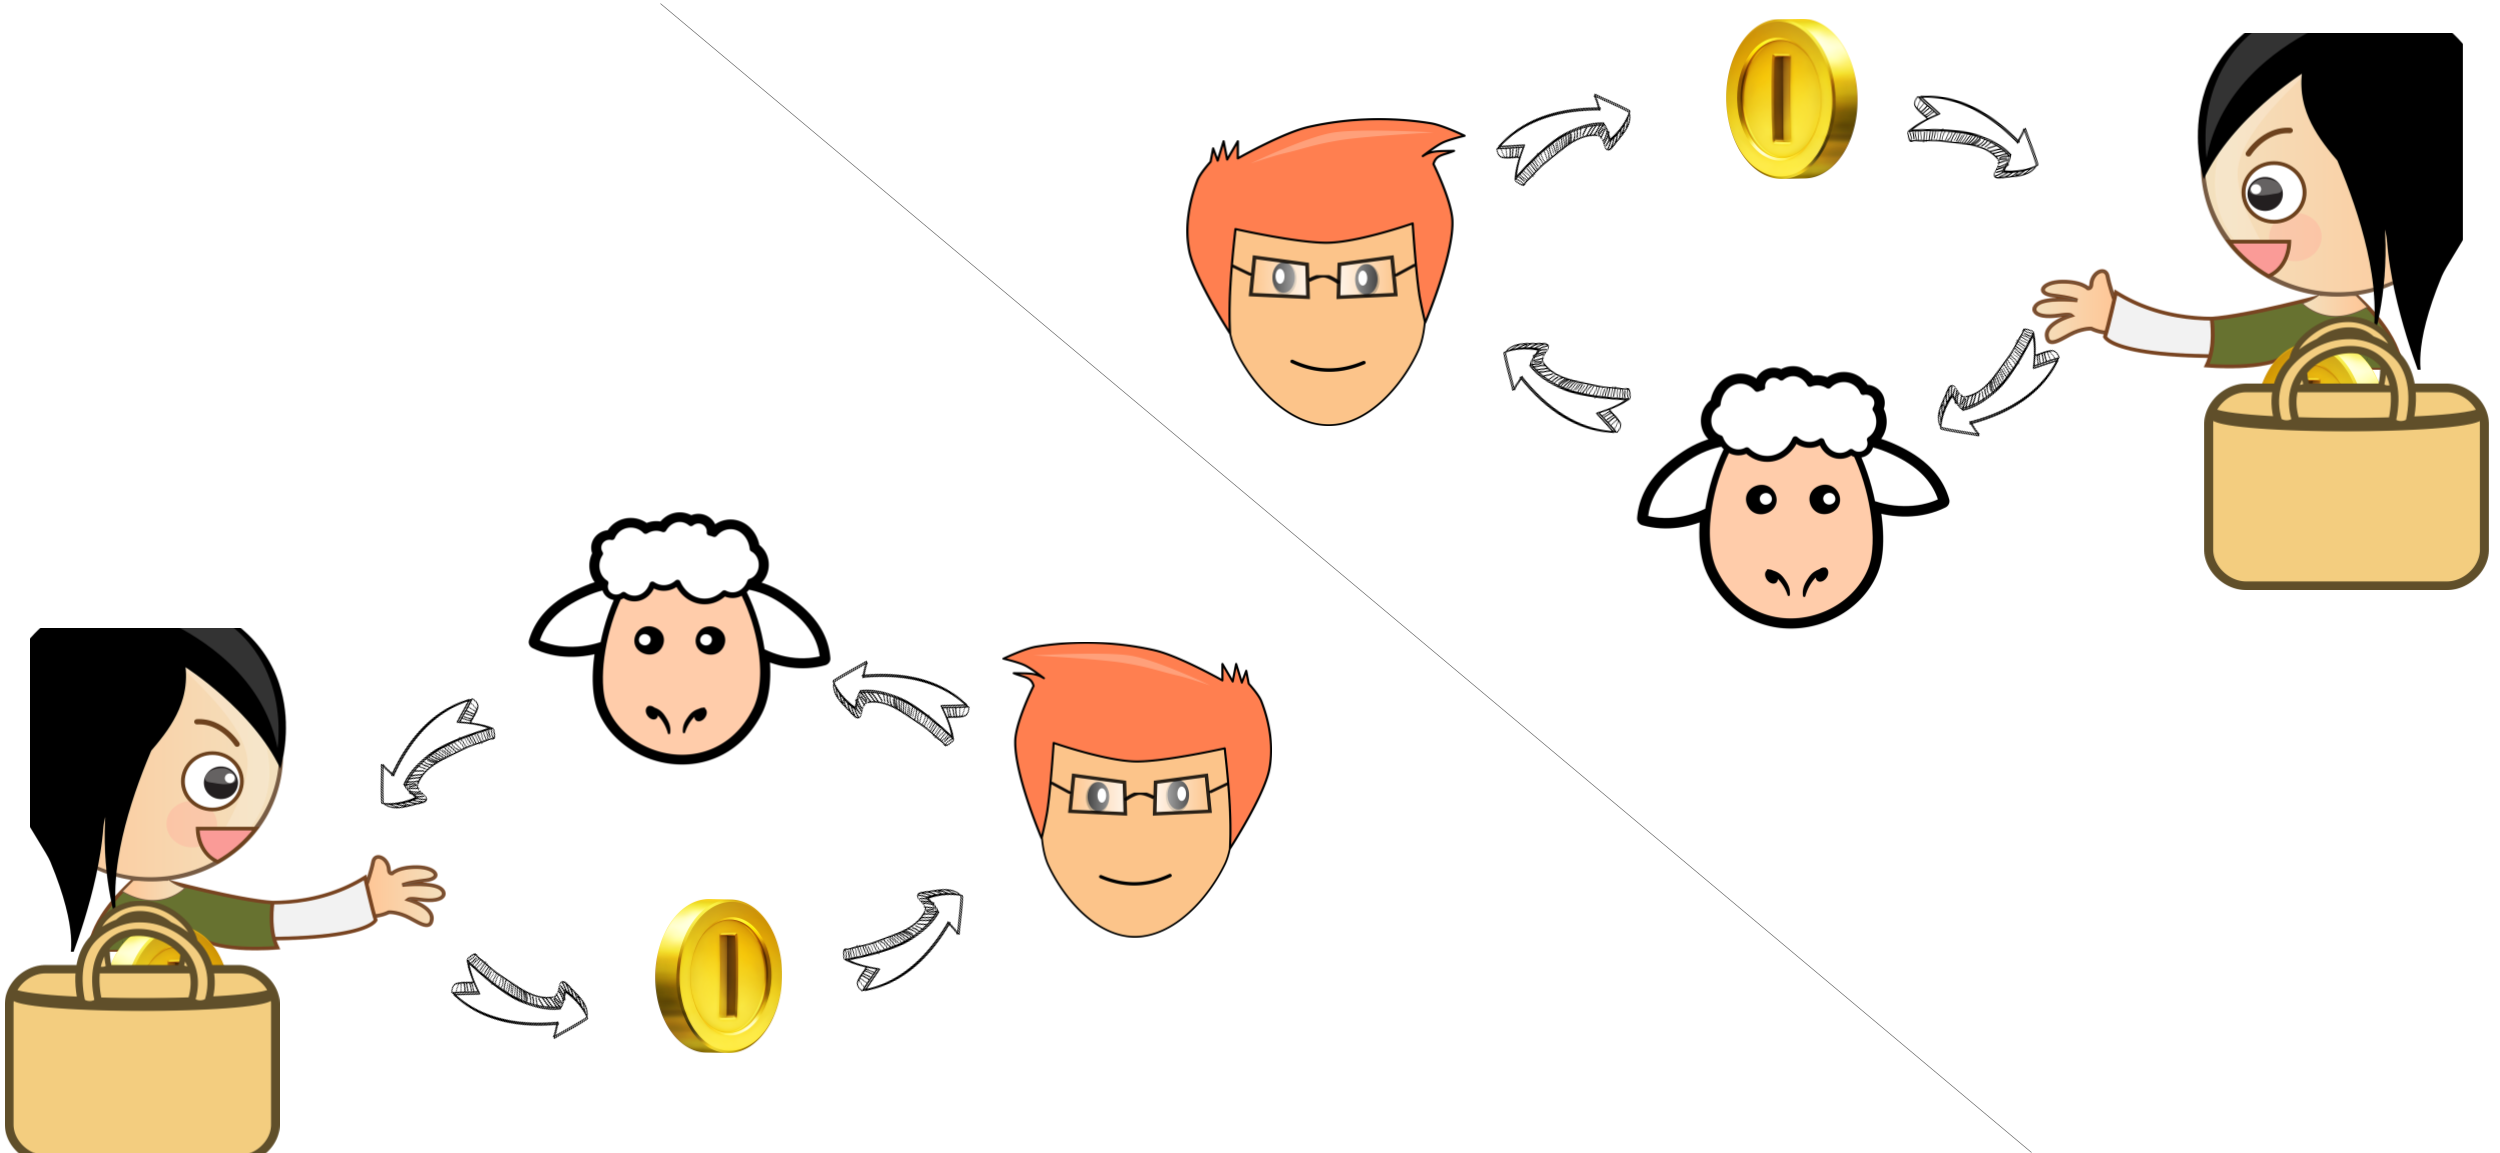
\includegraphics[scale=0.08]{./pics/used/sheep_example_HR}}
    \caption{Example for velocity}
    \label{fig:vola_example}
  \end{figure}

  $ \displaystyle
  \begin{aligned}%
    2 \coins \cdot V_{\mathtt{2019}} = %
    \begin{bmatrix}%
      1 \frac{\coins}{\sheep} \\%
      1 \frac{\coins}{\sheep}%
    \end{bmatrix} \cdot \begin{bmatrix}%
      1 \sheep & 1 \sheep%
    \end{bmatrix} = 2 \coins.%
  \end{aligned} %
  $ %

  $V_{\mathtt{2019}}= 1 = 0 \cdot \frac{%
    1\coins%
  }{%
    2\coins%
  } + 2 \cdot \frac{%
    1\coins%
  }{%
    2\coins%
  }$. %

  
\end{frame}


% -------------------------------------------------

\begin{frame}{... if things are easy -- let's just measure the thing!}
  \begin{align*}
    V_{\rho} = \frac{P_{\rho}T_{\rho}}{M_{\rho, \ttext{total}}}  
  \end{align*}

\end{frame}

% -------------------------------------------------

\begin{frame}{ Easy?... certainly not when dealing with blockchain!}

  \vfill

  \emphtext{Is change money ``transaction volume?''} %

  \vfill

  \blockquote[Fisher (1922)]{What is desired is the rate at which money is used for purchasing goods, not for making change.} %

  \vfill

  Change money? Aren't cryptocurrencies anonymous? Clustering? Heuristics? 

  \vfill
  
\end{frame}

% -------------------------------------------------

\begin{frame}{Technical Foundations: UTXO based cryptocurrencies}

  \begin{figure}
    \centerline{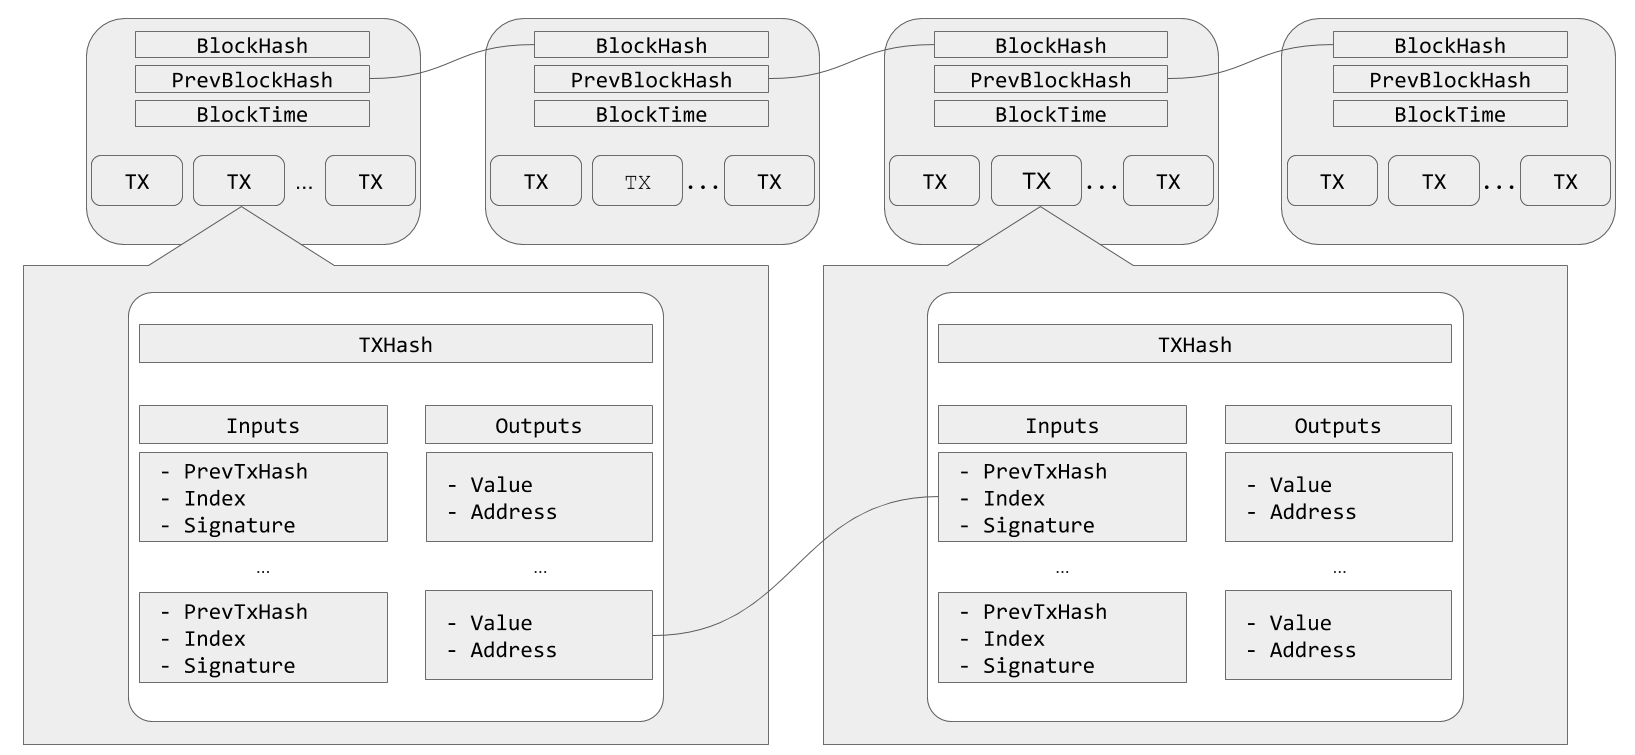
\includegraphics[scale=0.2]{./pics/used/utxo_sys_HR}}
    \caption{Blockchain and Transactions (Tschorsch et al. 2016, adjusted)}
    \label{fig:utxo_sys}
  \end{figure}

  
\end{frame}

% -------------------------------------------------

\begin{frame}{Technical Foundations: Clusterting}

  \begin{itemize}
  \item Statistical properties can be used to build clusters of addresses, %
    that are likely to belong to one individual user %
    (compare Meiklejohn, 2013)
  \item f.e. ``all inputs of a transaction most likely belong to one user''
  \item Here, just adoption of the approach of Kalodner (2018) 
  \end{itemize}
  
\end{frame}

% % -------------------------------------------------
% \begin{frame}{ Easy?... certainly not when dealing with blockchain!}
%   \vfill

%   \(P_{\rho}T_{\rho} = P'_{\rho}T'_{\rho} - C_{\rho}\)

%   \vfill

%   with

%   \begin{align*}
%     P'_{\rho}T'_{\rho} = \sum_{t = 1}^{T_{\rho}}\sum_{o=1}^{O_{\rho t}} \ttext{val}_{\rho t o}
%   \end{align*} %

%   and

%   \begin{align*}
%     C_{\rho} =  \sum_{t = 1}^{T_{\rho}} \sum_{c=1}^{C_{t}} \ttext{val}_{\rho t c} \text{ with } c \in C^{\ttext{selfchurn}} 
%   \end{align*}

% \end{frame}

% -------------------------------------------------

\begin{frame}{Velocity Estimators: Recent developments.}

  \begin{align*}
    V_{\ttext{naive}} = \frac{P'_{\rho}T'_{\rho}}{M_{\rho, \ttext{total}}}  
  \end{align*}
  
  \begin{itemize}
  \item Athey et al. (2016) \deemphtext{(Practically.)}
  \item Boldt and van Ordt (2016) \deemphtext{(Theoretic construction within a pricing model.)}
  \end{itemize}

  \begin{align*}
    V_{\ttext{total}} = \frac{P_{\rho}T_{\rho}}{M_{\rho, \ttext{total}}}
  \end{align*}

  \begin{itemize}
  \item Kalodner et al (2018) \deemphtext{(On the sidelines when introducing a new blockchain parser. But absolutly spot on!)}
  \end{itemize}
  
\end{frame}

% -------------------------------------------------

\begin{frame}{Problem solved?}
  \vfill
  Not quite!
  \vfill
  Velocity as \emphtext{merely scaled} version of the price-sum \(P_{\rho}T_{\rho}\) ?
  \vfill
  What about
  \begin{itemize}
  \item  ... broken money? (Meiklejohn, 2017) \deemphtext{(lost key, faulty transactions)}
  \item  ... Satoshi's Bitcoins?
  \item  ... long term investments? \deemphtext{(cold storage, ``hodling'')}
  \end{itemize}
  \visible<2->{
    \emphtext{What is money anyway?}
  }
  \vfill
\end{frame}

% -------------------------------------------------
\begin{frame}{Velocity Estimators: Velocity based on a segregated money supply}

  \centering{``all units issued are components of the money supply''}
  
  \centering{\emphtext{VS}}

  \centering{``money is what money does'' (Dalton, 1965)}%

  \vfill

  No fullfillment of the money functions by \emphtext{money hoards}.

\end{frame}

% -------------------------------------------------
\begin{frame}{Velocity Estimators: Velocity based on a segregated money supply}
  \begin{itemize}
    % \item No fullfillment of the money functions by \emphtext{money hoards}
  \item Hoarded money, as destroyed money, is \emphtext{``leakage''} that \emphtext{needs to be compensated} [Keynes (1973), Commons (1973)]
  \item Speculation might act as \emphtext{``regulator of the quantity of money.''} [Fisher (1911)]
  \item Law-of-Reflux [Fullarton (1845), populized by Marx (1872)]% as part of the ``anti-quantity theory of money''
    \begin{itemize}
    \item ``money taking the form of hoards'' and ``circulating'' money [Marx (1872)]
    \item illiquid component is seen as reservoir for money demand shocks
    \item excluded from money supply
    \end{itemize}
    % \item Hoarding might \emphtext{decrease the effective supply} in circulation and lead to feedback effects between speculation and prices [Athey et al. (2016) and Bolt et al. (2016)]
  \end{itemize}
\end{frame}

% -------------------------------------------------

\begin{frame}{Velocity Estimators: Velocity based on a segregated money supply}
  \begin{align*}
    V_{\ttext{total}, \rho} = v_{\rho z} \cdot \frac{N_{\rho z}}{\big( N_{\rho z}+\sum_{g=1}^{G_{\rho}} N_{\rho g} \big)} + \sum_{g=1}^{G_{\rho}} v_{\rho g} \cdot \frac{N_{\rho g}}{\big( N_{\rho z}+\sum_{g=1}^{G\rho} N_{\rho g} \big)}%
  \end{align*}
  \begin{align*}
    V_{\ttext{circ}, \rho} =  \sum_{g=1}^{G_{\rho}} v_{\rho g} \cdot \frac{N_{\rho g}}{\sum_{g=1}^{G_{\rho}} N_{\rho g} } = \emphtext{ \frac{P_{\rho}T_{\rho}}{M_{\rho, \ttext{circulating}}} }%
  \end{align*}
  \emphtext{\( z \)} denominating group of monetary units with zero turnover %

  \emphtext{\(N_{\rho g}\)} being  monetary units in group \(g\) for period \(\rho\) and

  \emphtext{\(v_{\rho g}\)} denominating group turnover numbers %


\end{frame}

% -------------------------------------------------

% \begin{frame}{Old and new interpretations.}

%   \emphtext{Assuming velocity increased...}

%   \vfill

%   Is money switching from ``hoarded'' to ``circulating ...?
%   ... or is money in circulation turned over more frequently?

%   \vfill

%   \begin{itemize}
%   \item \emphtext{Interpretation \(V_{\ttext{total}, \rho}\)} : average number of turnover all money units where able to achieve in period \(\rho\)
%   \item \emphtext{Interpretation \(V_{\ttext{circ}, \rho}\)} : average number of turnovers that effectively circulating money units where able to achieve in period \(\rho\)
%   \end{itemize}

%   \vfill

%   \emphtext{Changes in the  fraction of money in circulation are treated seperated from the turnover-characteristic of this money.}

% \end{frame}

% -------------------------------------------------

\begin{frame}{Velocity Estimators: A new estimator class}
  \vfill
  \begin{itemize}
  \item Calculate velocity for money in circulation exclusively
  \item ``Money circulating'' is defined \emphtext{wrt. to a certain time window}
  \end{itemize}
  \vfill
  \centering{\mbox{\Large $\Downarrow$}}
  \vfill
  \begin{itemize}
  \item Velocity becomes a \emphtext{function of the adopted time window length \(\alpha\)}.
  \item \deemphtext{Future research: Which window length leads to the best determinant of prices?}
  \end{itemize}
  \vfill
\end{frame}

% -------------------------------------------------

\begin{frame}{Velocity Estimators: Separating the money supply - Prerequisites}
  \begin{itemize}
  \item  Time window \(\Wndw\) covering \([\Wndw^\Start , \Wndw^\End]\), where \(\Wndw^\Start = \rho^{\End} - \alpha\) and \(\Wndw^\End = \rho^\End\) %
  \item General approach:
    \begin{itemize}
    \item Look at transactions in period \(\omega\)
    \item If UTXOs from pre-period \(\Rightarrow\) add to aggregate of money in circ.
    \item If UTXOs from within period \(\Rightarrow\) just a respent ``coin''.  
    \end{itemize}
  \end{itemize}
\end{frame}

%       % -------------------------------------------------

% \begin{frame}{Separating the money supply - Illustration}
%   \begin{figure}
%     \centerline{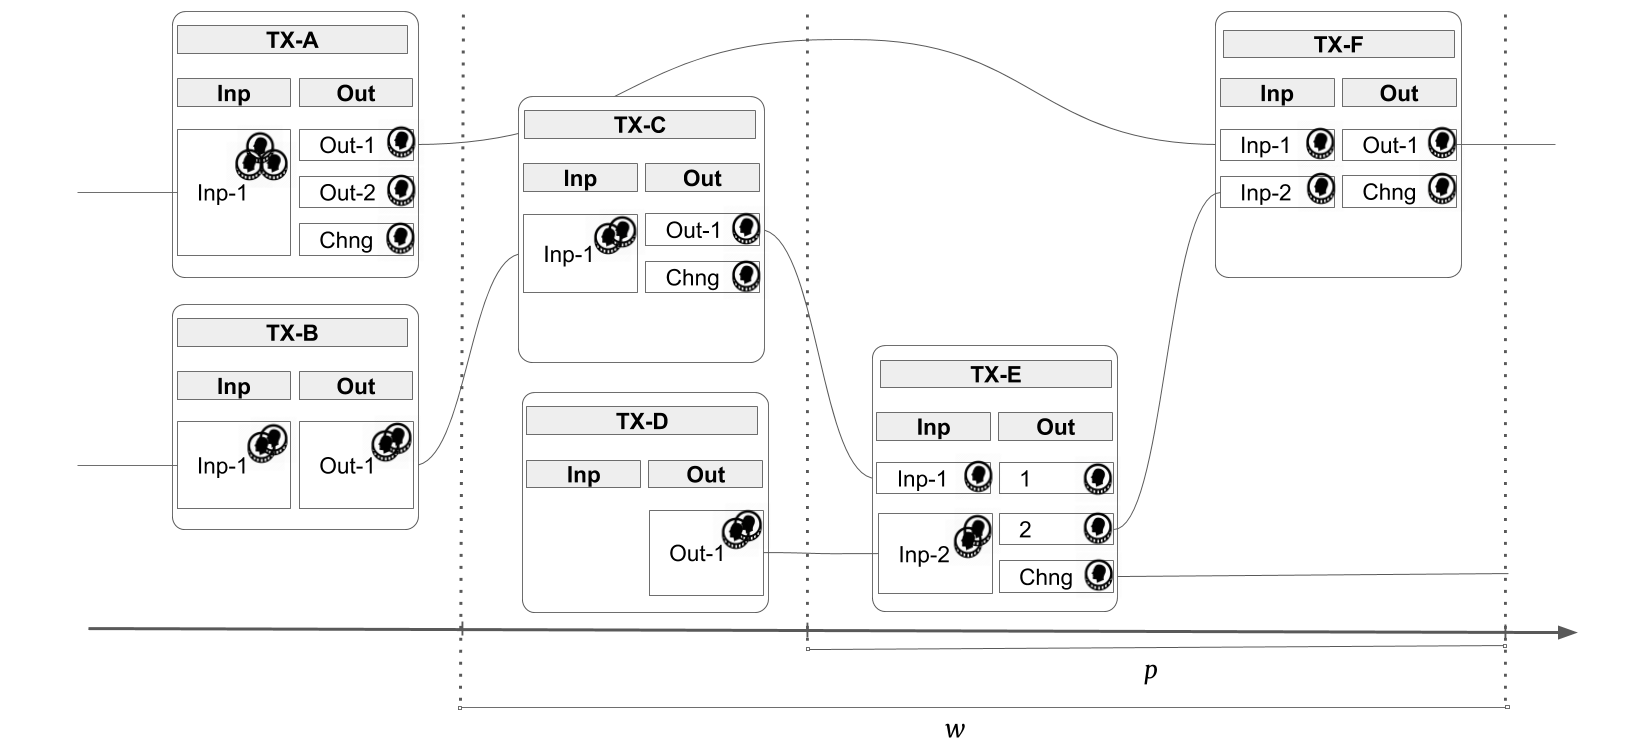
\includegraphics[scale=0.2]{../text/fig/mcirc_concept_window_uneqal_period_HR}}
%     \caption{An example of a transaction chain.}
%     \label{fig:mcirc_concept}
%   \end{figure}

% \end{frame}
%       % -------------------------------------------------

\begin{frame}{Velocity Estimators: Separating the money supply - Issues}
  Two major characteristics of UTXO-based cryptocurrencies shaping our approach: %
  \begin{enumerate}
  \item \emphtext{Transactions can spend inputs only in total}
    \begin{itemize}
    \item  Paying a Burger with a Bitcoin \(\Rightarrow\) Is change money to be counted?
    \item Two approaches: ``Whole-bill-approach'' or ``Moved-coin-approach''
    \end{itemize}
  \item \emphtext{The link between inputs and outputs of a transaction in indeterminable}
    \begin{itemize}
    \item Which input morves to the change output?
    \item Different assignment rules: ``LIFO'' vs ``FIFO''
    \end{itemize}
  \end{enumerate}
\end{frame}

%       % -------------------------------------------------

% \begin{frame}{Separating the money supply: Illustration}
%   \begin{figure}
%     \centerline{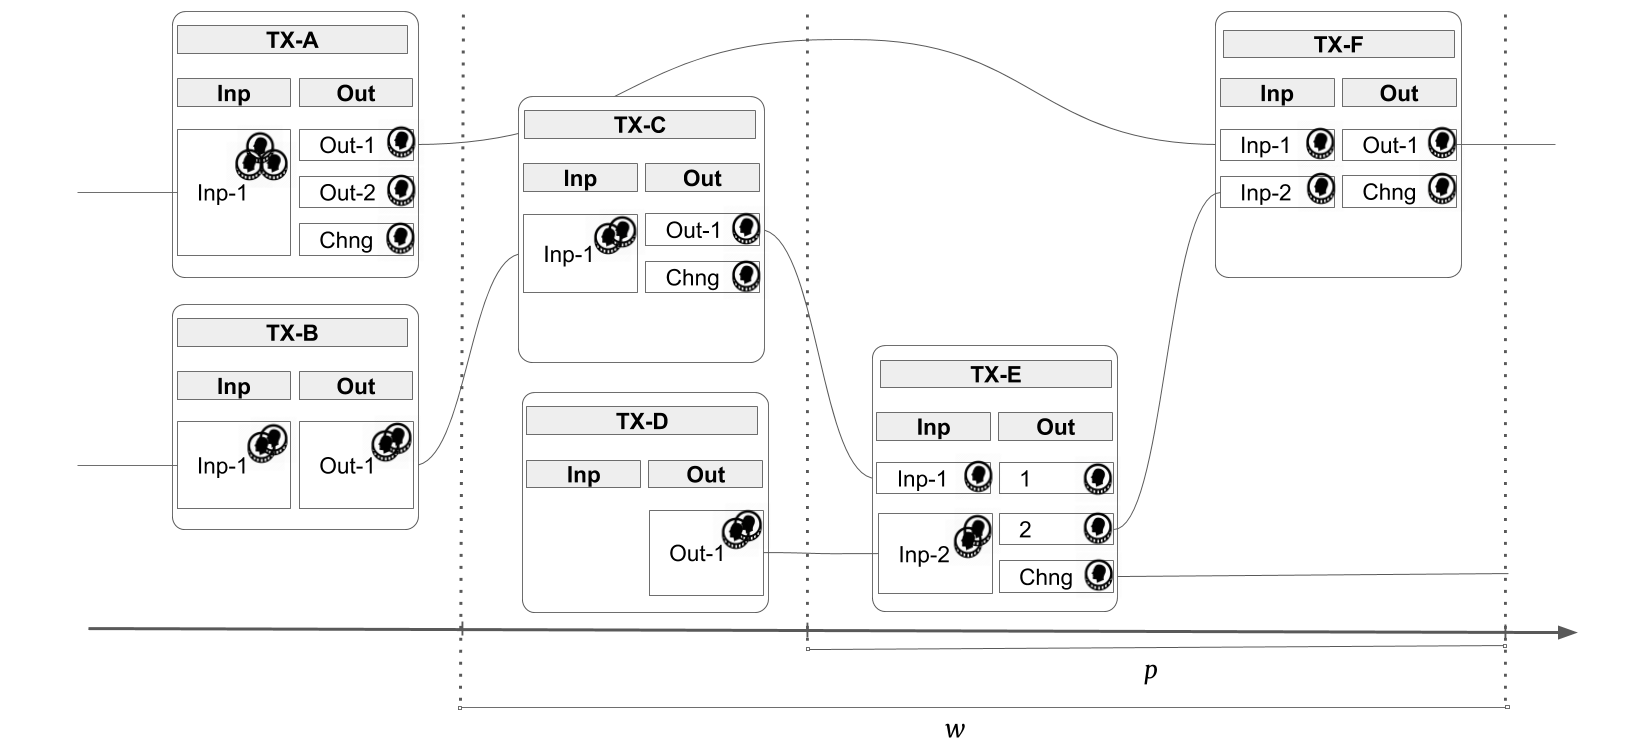
\includegraphics[scale=0.2]{../text/fig/mcirc_concept_window_uneqal_period_HR}}
%     \caption{An example of a transaction chain.}
%     \label{fig:mcirc_concept}
%   \end{figure}

% \end{frame}

%       % -------------------------------------------------

\begin{frame}{Velocity Estimators: Velocity measures based on circulating money supply}

  \emphtext{Measure 1: ``Whole-bill-approach''}
  \begin{align*}
    V_{\ttext{circWba}(\alpha) \rho} = \frac{P_{\rho}T_{\rho}}{M_{\rho}^{\ttext{circWba}(\alpha)}}.
  \end{align*}
  \emphtext{Measure 2: ``Moved-coin-approach'' - Type: ``First-in-first-out''} 
  \begin{align*}
    V_{\ttext{circMcaFifo}(\alpha) \rho} = \frac{P_{\rho}T_{\rho}}{M_{\rho}^{\ttext{circMcaFifo}(\alpha)}}
  \end{align*}
  \emphtext{Measure 3: ``Moved-coin-approach'' - Type: ``Last-in-first-out''} 

  \begin{align*}
    V_{\ttext{circMcaLifo}(\alpha) \rho} = \frac{P_{\rho}T_{\rho}}{M_{\rho}^{\ttext{circMcaLifo}(\alpha)}}.
  \end{align*}

  
\end{frame}

% -------------------------------------------------

\begin{frame}{Approximation methods: Overview}
  
  \begin{itemize}
  \item Number of transactions \linebreak[1]
    \deemphtext{Polasik et al. (2015)}
  \item Coin Days Destroyed \linebreak[1]
    \deemphtext{DeLeo and Stull (2014), Georgoula et al. (2015), Ciaian et al (2016), Kancs (2015), Bouoiyour and Selmi (2015)}
  \item Turnover \linebreak[1]
    \deemphtext{Smith (2017)}
  \end{itemize}
  
\end{frame}

% -------------------------------------------------

\begin{frame}{Approximation methods: Coin Days Destroyed and Turnover}

  \vfill

  \begin{itemize}
  \item \textbf{Coin days destroyed:}
    \begin{itemize}
    \item \emphtext{\textbf{\(V^{app}_{cdd}\)}}: \deemphtext{Accumulated over all spent outputs of period \(\rho\):} ``the \textbf{age} of as spent UTXO \textbf{multiplied with the value} of this output''
      
    \end{itemize}
    \item \textbf{Turnover:}
    \begin{itemize}
    \item \emphtext{\(V^{app}_{turn}\)}: ``Expected average turnover of coins in circulation''      
    \end{itemize}
  \end{itemize}
  \vfill
  
  % \begin{align*}
  %   \ttext{ctd}_{\rho t i} = \Delta t_{\rho t i} \cdot val^{input}_{\rho t i}
  % \end{align*}
  % For period \(\rho\) the ``coin-time-destroyed'' gets accumulated as
  % \begin{align}%
  %   \ttext{ctd}_{\rho} = \sum_{t=1}^{T_{ \rho}} \sum_{i=1}^{I_{\rho t}}  \ttext{ctd}_{\rho t i} .%
  % \end{align} %


  % \begin{align*}\label{eq:bdd}%
  %   \ttext{ctd}_{\rho} = \sum_{t=1}^{T_{\rho}}  \Delta t_{\rho t} \cdot \ttext{val}^{\ttext{tx}^{+}}_{\rho t},
  % \end{align*}%
  % where 
  % \begin{align*}
  %   \ttext{val}^{\ttext{tx}^{+}}_{\rho t} = \sum_{o=1}^{O_{\rho t}} \ttext{val}^{\ttext{output}}_{\rho t i} + \ttext{val}^{\ttext{fees}}_{\rho t} = \sum_{i=1}^{I_{\rho t}} \ttext{val}^{\ttext{input}}_{\rho t i}.
  % \end{align*}
  % and
  % \begin{align*}
  %   \Delta t_{\rho t} =  \sum_{i=1}^{I_{\rho t}} \Delta t_{\rho t i} \cdot \frac{\ttext{val}^{\ttext{input}}_{\rho t i}}{\sum_{i=1}^{I_{\rho t}} \ttext{val}^{\ttext{input}}_{\rho t i}}.
  % \end{align*}
  
\end{frame}

% -------------------------------------------------

% \begin{frame}{Approximation methods: Dormancy \& Turnover (Smith, 2018)}
%   \vfill
%   e usage''
%   \vfill
%   \vfill

%   %   \begin{align*}\label{eq:bdd}%
%                 %     \ttext{dorm}_{\rho}
%                 %   %     &= \frac{\ttext{ctd}_{\rho}}{\ttext{val}^{tx+}_{\rho}} \\ 
%                 %     &= \sum_{t=1}^{T_{\rho}}  \Delta t_{\rho t} \cdot \frac{\ttext{val}^{\ttext{tx}^{+}}_{\rho t}}{\ttext{val}^{tx+}_{\rho}},
%                 %   \end{align*}%
%                 % %   with
%                 % %   \begin{align*}
%                 %     %     \ttext{val}^{\ttext{tx}^{+}}_{\rho t} = \sum_{o=1}^{O_{\rho t}} \ttext{val}^{\ttext{output}}_{\rho t o} + \ttext{val}^{\ttext{fees}}_{\rho t} = \sum_{i=1}^{I_{\rho t}} \ttext{val}^{\ttext{input}}_{\rho t i}.
%                 %     %   \end{align*}
%                 %   with
%                 %   \begin{align*}
                        %                 %                         \Delta t_{\rho t} =  \sum_{i=1}^{I_{\rho t}} \Delta t_{\rho t i} \cdot \frac{\ttext{val}^{\ttext{input}}_{\rho t i}}{\sum_{i=1}^{I_{\rho t}} \ttext{val}^{\ttext{input}}_{\rho t i}}.
                        %                 %                       \end{align*}
                        %                 %                         \emphtext{\(\ttext{val}^{\ttext{input}}_{\rho t i}\)} being the input value of input \(i\) of transaction \(t\) of \(\rho\)

                        %                 %                         \emphtext{\(\ttext{val}^{tx+}_{\rho t}\)} being the volume of transact. \(t\) including transact. fees

                        %                 %                         \emphtext{\textbf{\(\frac{1}{\ttext{dorm}_{\rho}}\)}}: ``''

                        %                       \end{frame}

                        %                       -------------------------------------------------

\begin{frame}{Application case Bitcoin}
  \begin{itemize}
  \item Calculation of all proxy variable
  \item Calcualtion of Velocity based on total money supply (equivalent to time window = \(\alpha = \inf\))
  \item Calcualtion of Velocity based on money in circulation (time window = \(\alpha = 1 \ttext{ day}\))
  \item standardization $x^{stand} = \frac{x-\mu}{\sigma}$ and normalization $X^{norm} = \frac{X-X_{min}}{X_{max}-X_{min}}$.
  \item Evaluation of goodness of fit using MAE, MSE, MCS-tests and MZ-regressions
  \end{itemize}
\end{frame}




% -------------------------------------------------

\begin{frame}{Goodness of fit: MAE, MSE, MCS-tests}
  
  \begin{center}
    \begin{table}
      \caption{Mean absolute error for normalized data of %
        approximation methods compared to estimation methods. Approximators in %
        5\%-Model confidence set marked by \(\dag\) and %
        in 1\%-Model confidence set marked by \(\ddag\).}
      \inputTikZ{0.4}{../text/ts_tables/appVSest_errors_w_mcs.tex}
      \label{tbl: errortable1}
    \end{table}
    \vspace{-4mm}
  \end{center}

\end{frame}

% -------------------------------------------------

\begin{frame}{Goodness of fit: MZ-regressions}
  
  \begin{center}
    \begin{table}
      \caption{Minzer-Zarnowitz regressions for standardized and %
        normalized approximation and estimation data.}
      \inputTikZ{0.4}{../text/ts_tables/appVSest_mz_table.tex}
      \label{tbl: errortable2}
    \end{table}
    \vspace{-4mm}
  \end{center}

\end{frame}

% -------------------------------------------------

\begin{frame}{Conclusion}

  \begin{itemize}
  \item Complete analysis of concepts and practical approaches of velocity
  \item \emphtext{Unification \& replication} of all existing approximators and estimators
  \item \emphtext{Operationalization of a new velocity measure} accounting for ``hoarded'' money that doesn't do ``what money does''.
  \item \emphtext{Comparison} of approximators and estimators
    \begin{itemize}
    \item \emphtext{Superior approximation method:} The naive estimator 
    \item Even better: Use the data/code we are going to make public
    \end{itemize}
  \end{itemize}
  
\end{frame}

% -------------------------------------------------

\begin{frame}{APPENDIX: Separating the money supply: Illustration}
  \begin{figure}
    \centerline{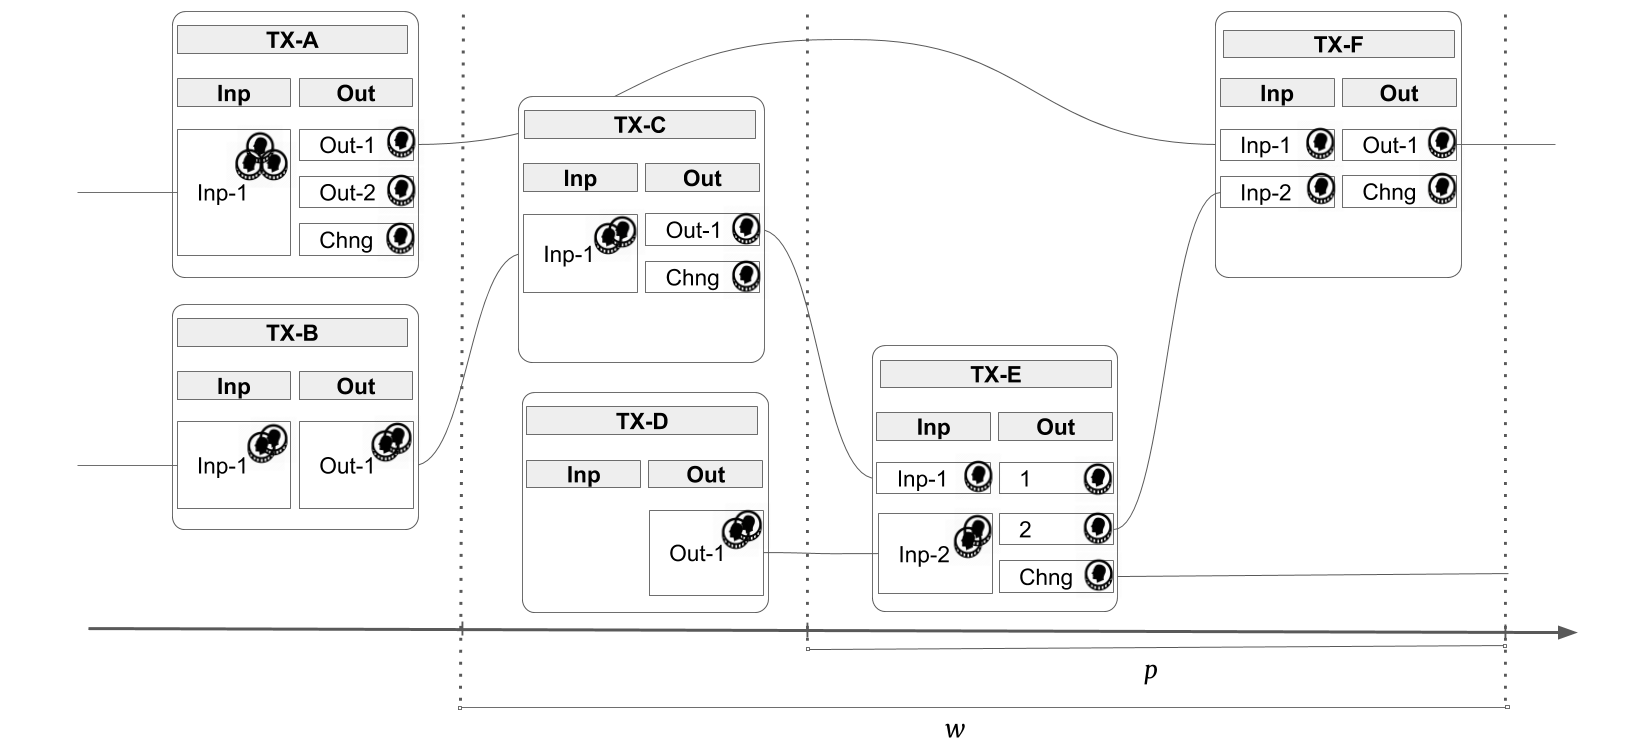
\includegraphics[scale=0.2]{../text/fig/mcirc_concept_window_uneqal_period_HR}}
    \caption{An example of a transaction chain.}
    \label{fig:mcirc_concept}
  \end{figure}

\end{frame}
% -------------------------------------------------

\begin{frame}{APPENDIX: Components of velocity estimates - Plot}
  \begin{figure}[h]
    \centering
    \inputTikZ{0.7}{../text/ts_figs/desc_components}
    \caption{Components of velocity estimators over time}
    \label{fig: Components of velocity estimators over time}
  \end{figure}

\end{frame}

% -------------------------------------------------

\begin{frame}{APPENDIX: Components of velocity estimates - Correlations}
  \begin{figure}[h]
    \centering
    \inputTikZ{0.55}{../text/ts_figs/corrplot_components.tex}
    \caption{Pearson correlations between the components of the velocity measures and the price in USD}
    \label{fig: Corrleation of components of velocity estimators}
  \end{figure}
\end{frame}


% -------------------------------------------------

\begin{frame}{Empirics of velocity approximators}
  \begin{figure}[h]
    \centering
    \inputTikZ{0.7}{../text/ts_figs/desc_all_app_norm}
    \caption{Velocity approximators (normalized) over time}
    \label{fig: Velocity approximators (normalized) over time}
  \end{figure}
\end{frame}
% -------------------------------------------------

\begin{frame}{Empirics of velocity approximators}
  \begin{figure}[h]
    \centering
    \inputTikZ{0.7}{../text/ts_figs/desc_all_app_stand}
    \caption{Velocity approximators (standardized) over time}
    \label{fig: Velocity approximators (standardized) over time}
  \end{figure}
\end{frame}
% -------------------------------------------------

\begin{frame}{Empirics of velocity estimators}
  \begin{figure}[h]
    \centering
    \inputTikZ{0.7}{../text/ts_figs/desc_all_est_norm}
    \caption{Velocity estimators (normalized) over time.}
    \label{fig: Velocity estimators (normalized) over time}
  \end{figure}
\end{frame}
% -------------------------------------------------

\begin{frame}{Empirics of velocity estimators}
  \begin{figure}[h]
    \centering
    \inputTikZ{0.7}{../text/ts_figs/desc_all_est_stand}
    \caption{Velocity estimators (standardized) over time}
    \label{fig: Velocity estimators (standardized) over time}
  \end{figure}
\end{frame}

% \begin{frame}{Discussion: Velocity as measure of ``moneyness''}

%   To what degree is a cryptocurrency used as medium-of-exchange?

%   \( \rightarrow \) \emphtext{``average coin turnover per period''} as a decent start

%   \begin{itemize}
%   \item ``Boom''
%     \begin{itemize}
%     \item Kept hot- or cold-wallets to wait for future price increases?
%     \item New speculators acting exclusivly on exchanges?
%     \end{itemize}
%   \item ``Bust''
%     \begin{itemize}
%     \item From wallet to exchange for selling them off?
%     \item Drawback of ``exchange-only'' speculators?
%     \end{itemize}  
%   \end{itemize}

% \end{frame}

%         % -------------------------------------------------

% \begin{frame}{Discussion: Velocity as measure of ``moneyness''}

%   \begin{itemize}



%   \item Character of these transactions:
%     \begin{itemize}
%     \item ``Portfolio management'' activities
%     \item Not indicating use as medium-of-exchange
%     \end{itemize}

%   \item Reflection on the blockchain:
%     \begin{itemize}
%     \item ``Sleep-hop-sleep patterns'' depending on market sentiment
%     \end{itemize}

%   \end{itemize}

% \end{frame}

%         % -------------------------------------------------

% \begin{frame}{Discussion: Velocity as measure of ``moneyness''}

%   \begin{itemize}
%   \item \emphtext{
%     Influence on \(V_{\ttext{total}, \rho} = \frac{P_{\rho}T_{\rho}}{M_{\rho, \ttext{total}}} \)}:

%     Transaction volume jumps but money supply stays constant.
%     \emph{Velocity increases.}

%   \item \emphtext{
%     Influence on \(V_{\ttext{circ}, \rho} = \frac{P_{\rho}T_{\rho}}{M_{\rho, \ttext{circulating}}} \)}:

%     Money in circulation increases, but it stays unused for performing additional peer-to-peer transactions.
%     \emph{Velocity decreases*.} 
%   \end{itemize}

%   * If the velocity was > 1 before the sentiment change.

% \end{frame}


\end{document}
